% Положения теории графов, используемые в разделе.
\subsection{Положения теории графов, используемые в главе}

Рассмотрим кубический плоский граф и вопросы его реберных раскрасок.
При этом, наряду с доказательствами существования самих раскрасок будем рассматривать алгоритмы построения этих раскрасок.
Сначала рассмотрим наиболее тривиальное утверждение.

\begin{lemma}\label{lem:text_3_graph_prim_coloring5}
Кубический граф допускает реберную раскраску в $5$ цветов, и эта раскраска может быть построена с линейной сложностью по количеству ребер.
\end{lemma}
Для построения требуемой раскраски достаточно последовательно перебрать все ребра.
Так как для каждого ребра существует ровно $4$ смежные ребра, то из пяти цветов всегда можно выбрать цвет, в который не покрашено ни одно из этих смежных ребер.
Таким образом, раскраска строится за один проход по всем ребрам, то есть с линейной сложностью.
$\blacksquare$\\

В лемме~\ref{lem:text_3_graph_prim_coloring5} не использовалась планарность графа, а количество цветов явно избыточно.
Согласно теореме Визинга \cite{Vizing1964}, \cite{Vizing1965} кубический граф допускает реберную раскраску в $4$ цвета.
Однако, теорема Визинга также не использует планарность графа, и алгоритм, построенный исходя из доказательсва, будет иметь сложность, выше линейной по количеству ребер \cite{Soifer2009}.
Приведем альтернативное доказательство с использованием планарности графа и более низкой сложностью алгоритма построения реберной раскраски в $4$ цвета.

\begin{theorem}\label{thr:text_3_graph_prim_coloring4}
Кубический граф допускает реберную раскраску в $4$ цвета, и эта раскраска может быть построена с линейной сложностью по количеству ребер.
\end{theorem}

Доказательство существования раскраски будем проводить по индукции по количеству вершин графа.
База индукции: кубический граф с минимальным количеством вершин это $K_4$.
Для этого графа утвержление очевидно.

Предположим, что утверждение теоремы верно для всех кубических графов с порядок которых изменяется от $4$ до $n - 2$ (отметим, что порядок кубического графа не может быть нечетным).

Рассмотрим кубический планарный граф, с множеством вершин $V$ ($n = |V| = \nu$), множеством ребер $E$ ($|E| = \epsilon$) и множеством граней $F$ ($|F| = \zeta$).
При этом внешнюю область вокруг графа также считаем гранью (рассматриваем граф, расположенный на сфере).
Также через $\zeta_i$ обозначим количество граней, содержашей ровно $i \ge 3$ вершин (в этом случае будем говорить, что грань имеет размер $i$).
\begin{equation}
	\zeta = \sum_{i = 3}^{\infty}{\zeta_i}.
\end{equation}
Рассмотрим соотношения, выполняемые для этого графа.

Так как степень каждой вершины равна $3$, то лемма о рукопожатиях для этого графа приобретает вид
\begin{equation}
	3 \nu = 2 \epsilon.
\end{equation}

Так как каждое ребро входит ровно в две грани, то верно соотношение
\begin{equation}
	2 \epsilon = \sum_{i = 3}^{\infty}{i \zeta_i}.
\end{equation}

Наконец, для рассматриваемого графа выполняется соотношение Эйлера $\nu + \zeta - \epsilon = 2$.
Подставив в соотношение Эйлера выражения для $\nu$, $\zeta$ и $\epsilon$ получим
\begin{equation}
	2 \cdot 2\epsilon + 6 \sum_{i = 3}^{\infty}{\zeta_i} - 3 \cdot 2\epsilon = 12
\end{equation}
\begin{equation}
	6 \sum_{i = 3}^{\infty}{\zeta_i} - \sum_{i = 3}^{\infty}{i \zeta_i} = 12
\end{equation}
\begin{equation}\label{eqn:text_3_graph_prim_euler}
	\sum_{i = 3}^{\infty}{(6 - i) \zeta_i} = 12
\end{equation}

Из \eqref{eqn:text_3_graph_prim_euler} видно, что в рассматриваемом графе найдется грань размера $3$, $4$ или $5$.
Рассмотрим каждый этих случаев отдельно.

Случай 1. В графе найдется треугольная грань.

\begin{figure}[ht]
	\centering
		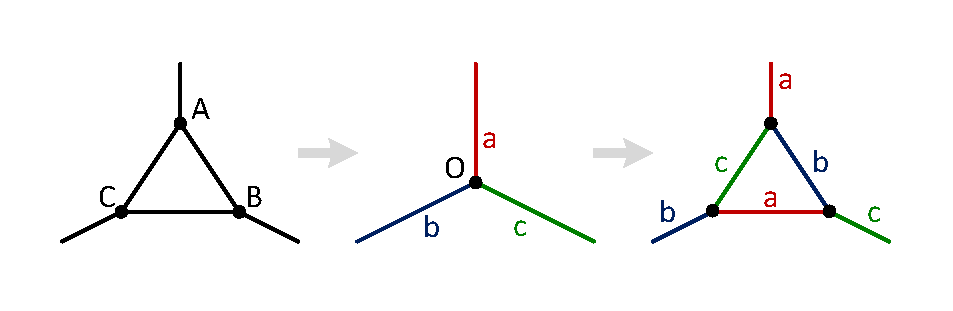
\includegraphics[width=1.0\textwidth]{./pics/text_3_graph_prim/coloring4_face3.pdf}
	\caption{}
	\label{fig:text_3_graph_prim_coloring4_face3}
\end{figure}

Случай 2. В графе нет треугольных граней, но найдется четырехугольная грань.

\begin{figure}[ht]
	\centering
		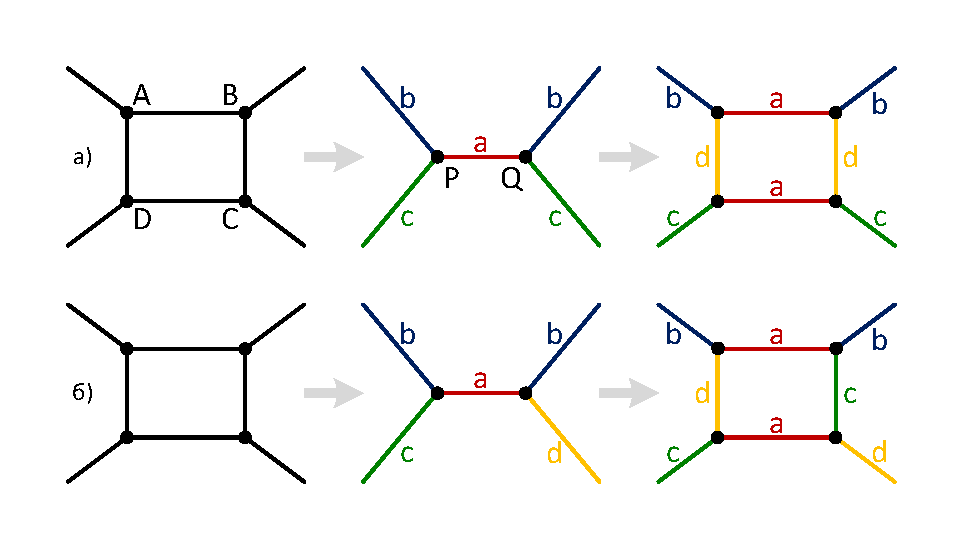
\includegraphics[width=1.0\textwidth]{./pics/text_3_graph_prim/coloring4_face4.pdf}
	\caption{}
	\label{fig:text_3_graph_prim_coloring4_face4}
\end{figure}

Случай 3. В графе нет треугольных и четырехугольных граней, но найдется пятиугольная грань.

$\blacksquare$\\